\chapter{Química dos heterociclos}\label{ch:b3:heterocycles}

Uma xícara de café contém cafeína, construída a partir de dois anéis fundidos que contêm quatro
átomos de nitrogênio, e seu aroma vem de dezenas de furanos, pirróis, pirazinas
e tiofenos formados na torrefação. A maioria dos fármacos da prateleira de uma farmácia contém pelo
menos um anel com um átomo de nitrogênio, oxigênio ou enxofre, assim como as bases
do DNA, o \omterm{def:b3:bioinorganic:haem}{heme}, a clorofila e muitas vitaminas. Este capítulo explica como um
heteroátomo em um anel aromático modifica seus elétrons: ele pode tornar o anel
mais pobre ou mais rico que o benzeno, e isso decide onde e como ele reage. O capítulo
termina com três maneiras clássicas de construir esses anéis.

\begin{recall}
O volume do 2.º ano tratou da aromaticidade e da regra de Hückel, dos arenos e da
substituição eletrofílica aromática pelo intermediário de Wheland, dos grupos
ativantes e orientadores, das aminas e de sua basicidade, das iminas, das enaminas,
dos tautômeros e das nucleobases; o volume do 1.º ano, do $\mathrm pK_a$, dos nucleófilos, dos
eletrófilos e dos grupos de saída. O \cref{ch:b3:pericyclic} deu o \omterm{def:b3:pericyclic:families}{rearranjo sigmatrópico}
[3,3].
\end{recall}

\begin{omfigure}
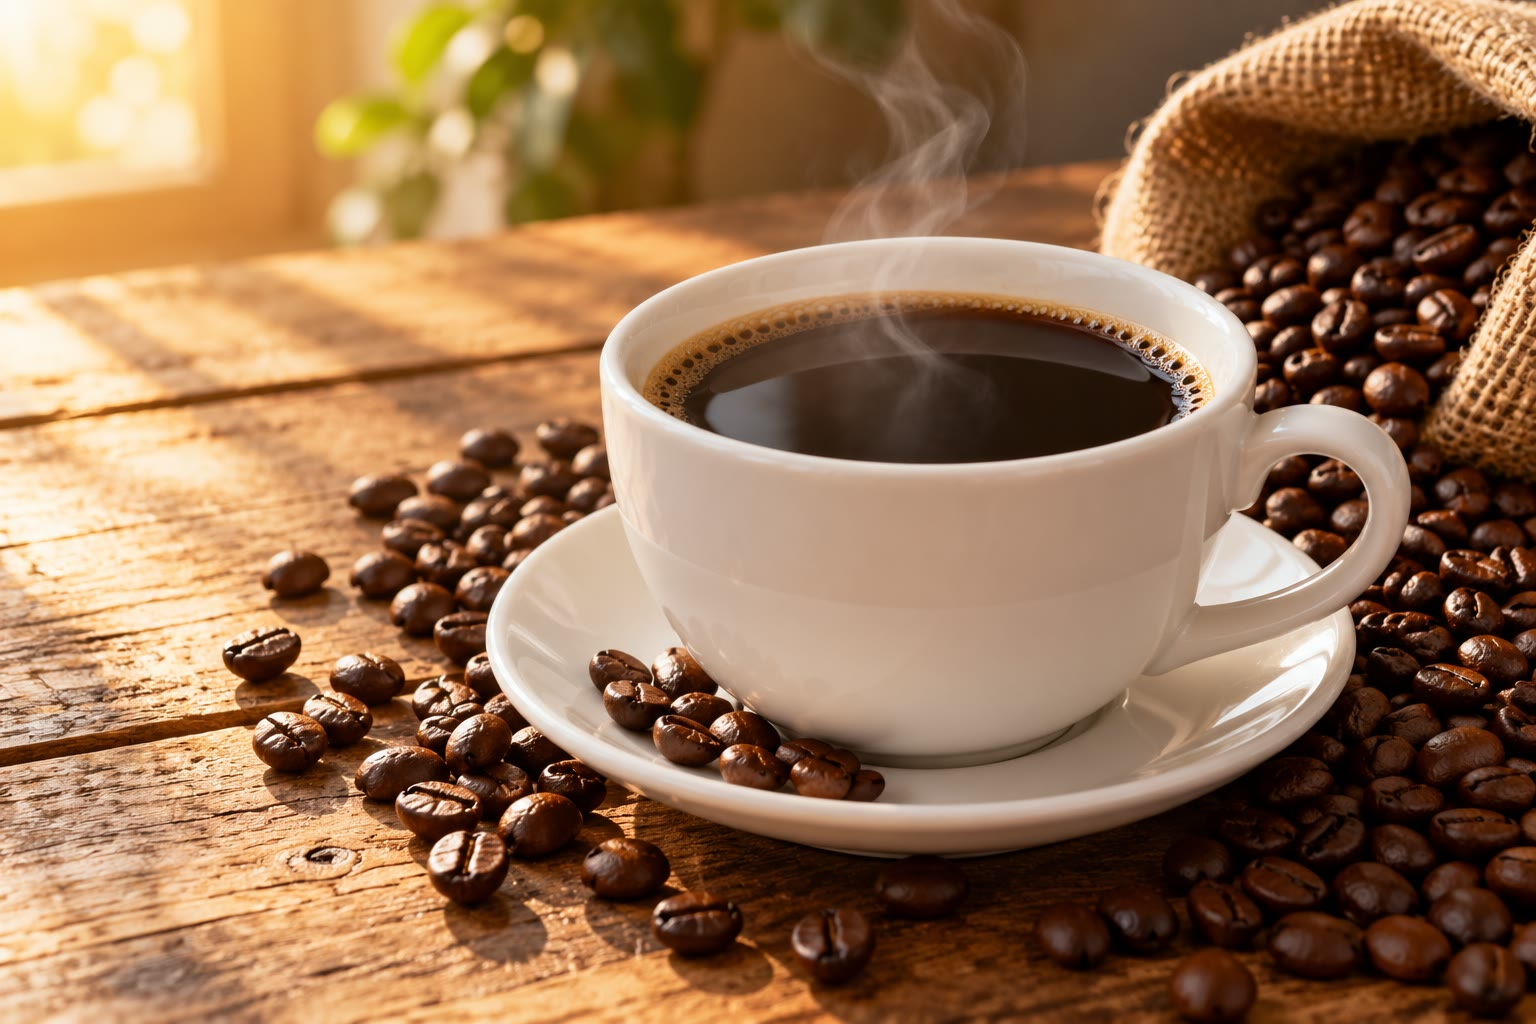
\includegraphics[width=0.5\linewidth]{images/book4/ai/b3-29-coffee.jpg}

{\small Uma xícara de café e grãos torrados: a cafeína, uma purina, e muitas das
moléculas de aroma formadas na torrefação são \omterm{def:b3:heterocycles:heterocycle}{heterociclos}.}
\end{omfigure}

\section{Heterociclos aromáticos}

\begin{definition}[Heterociclos]\label{def:b3:heterocycles:heterocycle}
Um \emph{heterociclo}\index{heterociclo} é um composto cíclico com pelo menos um
átomo diferente do carbono no anel; um \emph{composto
heteroaromático}\index{composto heteroaromatico@composto heteroaromático} é um heterociclo aromático, como a piridina, o
pirrol, o furano ou o tiofeno.
\end{definition}

\begin{proposition}[Seis elétrons $\pi$]\label{prop:b3:heterocycles:sextet}
A piridina, o pirrol, o furano, o tiofeno e o imidazol têm, cada um, seis elétrons $\pi$ em
um anel plano, cíclico e conjugado, e são aromáticos pela regra de Hückel.
\end{proposition}

\begin{proof}
Piridina: os cinco carbonos e o nitrogênio dão, cada um, um elétron p; o par isolado do
nitrogênio está em um orbital $sp^2$ no plano do anel, fora do sistema $\pi$: $5 + 1 = 6$.
Pirrol: os quatro carbonos dão um cada, e o nitrogênio, ligado a H no plano,
põe seu par isolado em seu orbital p: $4 + 2 = 6$. Furano e tiofeno: como o pirrol, o
heteroátomo cede um de seus dois pares isolados (o outro fica no plano). Imidazol:
o nitrogênio N--H dá dois, o nitrogênio do tipo piridina um, os três carbonos,
três: 6. Seis é $4n + 2$ com $n = 1$.
\end{proof}

\begin{omfigure}
\begin{tikzpicture}[font=\small, yscale=0.55]
  % pyridine: six p orbitals perpendicular to the ring (drawn first), N at 0 deg
  \foreach \a in {0,60,...,300} { \pic at (\a:1.1) {omp={0.62}{90}}; }
  \draw[thick] (0:1.1) -- (60:1.1) -- (120:1.1) -- (180:1.1) -- (240:1.1) -- (300:1.1) -- cycle;
  \node[fill=white, inner sep=0.5pt] at (0:1.1) {N};
  \pic at ($(0:1.1)+(0.2,0)$) {omlobe={0.8}{0}};
  \node[font=\scriptsize, align=center, anchor=north] at (0,-2.4) {piridina: 6 elétrons p de 6 átomos;\\ par isolado no plano (básico)};
  \begin{scope}[xshift=5.4cm]
    \foreach \a in {0,72,144,216,288} { \pic at (\a:1.0) {omp={0.62}{90}}; }
    \draw[thick] (0:1.0) -- (72:1.0) -- (144:1.0) -- (216:1.0) -- (288:1.0) -- cycle;
    \node[fill=white, inner sep=0.5pt] at (0:1.0) {N};
    \draw ($(0:1.0)+(0.18,0)$) -- (0:1.7) node[right, inner sep=0.5pt] {H};
    \node[font=\scriptsize, align=center, anchor=north] at (0,-2.4) {pirrol: o par isolado de N é um dos\\ 6 elétrons $\pi$ (não básico)};
  \end{scope}
\end{tikzpicture}

{\small Os sistemas $\pi$ da piridina e do pirrol, vistos obliquamente: um orbital p por
átomo do anel, perpendicular ao anel. Na piridina, o par isolado do nitrogênio (o lobo no plano, no
nitrogênio) aponta para fora no plano do anel e está livre para ligar um próton; no pirrol,
o nitrogênio, que porta um hidrogênio no plano, cede seu par isolado ao
sexteto aromático.}
\end{omfigure}

\begin{definition}[Heterociclos $\pi$-excedentes e $\pi$-deficientes]\label{def:b3:heterocycles:pi-character}
Um \emph{heterociclo $\pi$-excedente}\index{heterociclo pi-excedente@heterociclo $\pi$-excedente}, como o
pirrol, o furano ou o tiofeno, tem seis elétrons $\pi$ em cinco átomos e uma \omterm{def:b3:computational-chemistry:dft}{densidade
eletrônica} $\pi$ em seus carbonos maior que a do benzeno; um \emph{heterociclo
$\pi$-deficiente}\index{heterociclo pi-deficiente@heterociclo $\pi$-deficiente}, como a piridina, tem um
átomo eletronegativo no anel que retira densidade $\pi$ dos carbonos.
\end{definition}

\begin{proposition}[Basicidade]\label{prop:b3:heterocycles:basicity}
A piridina é uma base moderada e o pirrol quase não é básico; o pirrol, quando é
protonado em ácido forte, recebe o próton no carbono, e não no nitrogênio.
\end{proposition}

\begin{proof}[Argumento]
% ledger: pka:pyridinium, pka4:pyrrolium, pka4:piperidinium, pka4:imidazolium, pka4:DMAPH
O par isolado da piridina está fora do sistema $\pi$: protoná-lo não custa
aromaticidade, e o piridínio tem $\mathrm pK_a = 5.2$; ela é menos básica que a piperidina
(o nitrogênio do piridínio é $sp^2$, com mais caráter s, e retém seu par mais
firmemente: piperidínio 11.1). Protonar o nitrogênio do pirrol tiraria seu par isolado
do sexteto e destruiria a aromaticidade; só ácidos muito fortes
protonam o pirrol, em C2, onde o cátion conserva alguma deslocalização
($\mathrm pK_a$ de cerca de $-4$). O imidazol tem os dois tipos de nitrogênio: ele é protonado no
nitrogênio do tipo piridina, e seu cátion, simétrico, é estabilizado por ressonância ($\mathrm pK_a$
7.0), a razão pela qual a histidina atua como ácido e como base nas \omterm{def:b3:complex-kinetics:enzyme}{enzimas}.
A 4-(dimetilamino)piridina é ainda mais básica ($\mathrm pK_a$ 9.6): o grupo amino empurra
seu par isolado para o anel e até o nitrogênio do anel.
\end{proof}

% ledger: dip:pyridine, dip4:pyrrole, dip4:furan, dip4:thiophene
Os momentos dipolares contam a mesma história: a piridina (\qty{2.19}{D}) tem sua extremidade negativa
no nitrogênio, enquanto no pirrol (\qty{1.84}{D}) a doação do par isolado ao anel
põe a extremidade negativa no anel e a positiva no nitrogênio. No furano
(\qty{0.66}{D}) e no tiofeno (\qty{0.55}{D}), os dois efeitos, retirada $\sigma$ e doação $\pi$, quase se
cancelam.

\begin{omfigure}
% ledger: h1:pyridine.a, h1:pyridine.g, h1:pyridine.b, h1:pyrrole.a, h1:pyrrole.b, h1:pyrrole.NH, h1:furan.a, h1:furan.b
\begin{tikzpicture}
\begin{axis}[width=0.86\linewidth, height=6.2cm, x dir=reverse, xmin=5.8, xmax=9.0, ymin=-0.1, ymax=3.6,
  axis x line=bottom, axis y line=none, xlabel={$\delta$ / ppm}, tick label style={font=\scriptsize}, label style={font=\small}]
\addplot[omDef, thick] table[x=ppm, y expr=\thisrow{y}+2.4] {figdata/out/bachelor-3-heterocycle-nmr-pyridine.dat};
\addplot[omThm, thick] table[x=ppm, y expr=\thisrow{y}+1.2] {figdata/out/bachelor-3-heterocycle-nmr-pyrrole.dat};
\addplot[omMeth, thick] table[x=ppm, y=y] {figdata/out/bachelor-3-heterocycle-nmr-furan.dat};
\node[font=\scriptsize, omDef, anchor=west] at (axis cs:6.6,3.0) {\shortstack[l]{piridina: H2/6, H4,\\ H3/5 (2\,:\,1\,:\,2)}};
\node[font=\scriptsize, omThm, anchor=west] at (axis cs:7.7,1.8) {pirrol: NH, H2/5, H3/4};
\node[font=\scriptsize, omMeth, anchor=west] at (axis cs:7.2,0.6) {furano: H2/5, H3/4};
\end{axis}
\end{tikzpicture}

{\small RMN de prótons da piridina, do pirrol e do furano em clorofórmio deuterado,
sintetizada a partir de deslocamentos medidos como linhas simples (acoplamentos omitidos), com
áreas iguais aos números de prótons. A piridina, $\pi$-deficiente, tem seus sinais H2/6 e H4
bem a campo baixo em relação ao do benzeno; o pirrol e o furano, $\pi$-excedentes, têm a maioria
dos seus a campo alto em relação a ele; os prótons vizinhos ao heteroátomo são sempre os mais
desblindados.}
\end{omfigure}

\section{A piridina}

A piridina resiste à substituição eletrofílica: o eletrófilo encontra um anel
mais pobre em elétrons que o benzeno e, no ácido em geral presente, um
íon piridínio cuja carga positiva o repele. A nitração exige condições muito
drásticas e dá o isômero 3 com baixo rendimento.

\begin{proposition}[Substituição eletrofílica em C3]\label{prop:b3:heterocycles:pyridine-c3}
O ataque eletrofílico à piridina ocorre em C3: o ataque em C2 ou C4 dá um
intermediário de Wheland do qual uma das estruturas de ressonância põe a carga positiva
no nitrogênio, com apenas seis elétrons ao seu redor.
\end{proposition}

\begin{proof}
No cátion do ataque em C2 (ou C4), a carga positiva se distribui sobre C3, C5
e N1 (ou C3, C5 e N1): uma estrutura de ressonância com um nitrogênio deficiente em elétrons,
de seis elétrons, muito desfavorável para um átomo eletronegativo. O ataque
em C3 distribui a carga apenas sobre C2, C4 e C6. Os três cátions são todos menos estáveis
que o do benzeno, mas o ataque em C3 é o menos ruim.
\end{proof}

\begin{definition}[N-óxido de piridina]\label{def:b3:heterocycles:n-oxide}
Um \emph{N-óxido de piridina}\index{N-oxido de piridina@N-óxido de piridina}, preparado pela oxidação da piridina
com um perácido, tem um grupo $\mathrm{N^+{-}O^-}$ cujo oxigênio devolve elétrons a C2
e C4; ele sofre substituição eletrofílica em C4, e o oxigênio é depois
removido.
\end{definition}

\begin{definition}[Substituição nucleofílica aromática]\label{def:b3:heterocycles:snar}
A \emph{substituição nucleofílica aromática}\index{substituicao nucleofilica aromatica@substituição nucleofílica aromática}
($\mathrm S_\mathrm NAr$) substitui um grupo de saída em um anel aromático pobre em elétrons
por um nucleófilo, por adição seguida de eliminação. O intermediário de adição
aniônico é um \emph{complexo de Meisenheimer}\index{complexo de Meisenheimer}.
\end{definition}

\begin{proposition}[$\mathrm S_\mathrm NAr$ em C2 e C4]\label{prop:b3:heterocycles:snar-positions}
As halopiridinas sofrem $\mathrm S_\mathrm NAr$ facilmente em C2 e C4 e apenas lentamente em C3,
porque a adição em C2 ou C4 põe a carga negativa no nitrogênio.
\end{proposition}

\begin{proof}
A adição em C2 torna C2 $sp^3$ e deixa quatro elétrons $\pi$ mais o par que entra
distribuídos sobre N1, C3 e C5 (ou, para C4: C3, C5 e N1): uma estrutura de ressonância tem a
carga negativa no nitrogênio eletronegativo. A adição em C3 a distribui apenas sobre
C2, C4 e C6, todos carbonos.
\end{proof}

\begin{omfigure}
\begin{tikzpicture}[font=\small, >=Stealth]
  \draw[thick] (-0.000,-0.620) -- (0.537,-0.310) -- (0.537,0.310) -- (0.000,0.620) -- (-0.537,0.310) -- (-0.537,-0.310) -- cycle;
  \draw[thick] (0.082,-0.424) -- (0.326,-0.283);
  \draw[thick] (0.326,0.283) -- (0.082,0.424);
  \draw[thick] (-0.408,0.141) -- (-0.408,-0.141);
  \node[fill=white, inner sep=0.4pt, font=\scriptsize] at (-0.000,-0.620) {N};
  \draw (0.537,-0.310) -- (0.927,-0.535) node[right, inner sep=0.5pt, font=\scriptsize] {Cl};
  \draw[thick] (3.400,-0.620) -- (3.937,-0.310) -- (3.937,0.310) -- (3.400,0.620) -- (2.863,0.310) -- (2.863,-0.310) -- cycle;
  \draw[thick] (3.726,0.283) -- (3.482,0.424);
  \draw[thick] (2.992,0.141) -- (2.992,-0.141);
  \node[fill=white, inner sep=0.4pt, font=\scriptsize] at (3.400,-0.620) {N};
  \node[font=\scriptsize, omThm] at (3.350,-0.920) {$\ominus$};
  \draw (3.937,-0.310) -- (4.386,-0.343) node[right, inner sep=0.5pt, font=\scriptsize] {Nu};
  \draw (3.937,-0.310) -- (4.190,-0.682) node[right, inner sep=0.5pt, font=\scriptsize] {Cl};
  \draw[thick] (6.800,-0.620) -- (7.337,-0.310) -- (7.337,0.310) -- (6.800,0.620) -- (6.263,0.310) -- (6.263,-0.310) -- cycle;
  \draw[thick] (6.882,-0.424) -- (7.126,-0.283);
  \draw[thick] (7.126,0.283) -- (6.882,0.424);
  \draw[thick] (6.392,0.141) -- (6.392,-0.141);
  \node[fill=white, inner sep=0.4pt, font=\scriptsize] at (6.800,-0.620) {N};
  \draw (7.337,-0.310) -- (7.727,-0.535) node[right, inner sep=0.5pt, font=\scriptsize] {Nu};
  \draw[->, thick] (1.25,0) -- (2.35,0) node[midway, above, font=\scriptsize] {$+\,\mathrm{Nu^-}$};
  \draw[->, thick] (4.65,0) -- (5.75,0) node[midway, above, font=\scriptsize] {$-\,\ce{Cl-}$};
  \node[font=\scriptsize] at (3.4,-1.2) {complexo de Meisenheimer};
\end{tikzpicture}

{\small Substituição nucleofílica da 2-cloropiridina: o nucleófilo se adiciona a
C2, dando um intermediário aniônico cuja carga negativa fica em grande parte no
nitrogênio do anel (uma estrutura de ressonância mostrada); o cloreto sai então e o
anel aromático é restaurado.}
\end{omfigure}

\begin{proposition}[Adição--eliminação]\label{prop:b3:heterocycles:snar-mechanism}
Para uma reação $\mathrm S_\mathrm NAr$ cuja etapa de adição é determinante da velocidade, $v = k[\mathrm{ArX}][\mathrm{Nu^-}]$,
e o fluoreto é o melhor grupo de saída entre os haletos.
\end{proposition}

\begin{proof}[Argumento]
A velocidade é a da adição bimolecular. A ligação carbono--halogênio não é
rompida nessa etapa; o que importa é quanto o halogênio abaixa a energia do
estado de transição aniônico retirando elétrons, e o flúor, o mais
eletronegativo, é o que mais o faz: a ordem F $>$ Cl $\approx$ Br $>$ I, oposta à da $\mathrm S_\mathrm N2$.
\end{proof}

\begin{definition}[Reação de Chichibabin]\label{def:b3:heterocycles:chichibabin}
A \emph{reação de Chichibabin}\index{reacao de Chichibabin@reação de Chichibabin} é a aminação da
piridina em C2 pela amida de sódio: o íon amideto se adiciona a C2, e um íon hidreto é
perdido, como di-hidrogênio após reação com o produto.
\end{definition}

A piridina e a DMAP servem também como bases e como catalisadores nucleofílicos: nas
acilações com anidridos de ácido, a DMAP ataca primeiro o anidrido, dando um
íon acilpiridínio que transfere seu grupo acila ao álcool muito mais depressa que
o próprio anidrido. As piridinas, as bipiridinas e as fenantrolinas estão entre os
ligantes mais comuns da química de coordenação.

\section{Anéis de cinco membros}

\begin{proposition}[Substituição eletrofílica do pirrol em C2]\label{prop:b3:heterocycles:pyrrole-c2}
O pirrol, o furano e o tiofeno sofrem substituição eletrofílica sobretudo em C2,
porque o cátion do ataque em C2 tem três estruturas de ressonância e o
do ataque em C3, apenas duas.
\end{proposition}

\begin{proof}
Após o ataque em C2, a carga positiva pode ficar em C3, em C5 ou no nitrogênio,
onde é compartilhada por meio do par isolado e todo átomo conserva um octeto (terceira
estrutura). Após o ataque em C3, ela pode ficar apenas em C2 ou no nitrogênio: a carga
é menos deslocalizada (ver a figura).
\end{proof}

\begin{omfigure}
\begin{tikzpicture}[font=\small]
  \draw[thick] (0.000,0.620) -- (0.590,0.192) -- (0.364,-0.502) -- (-0.364,-0.502) -- (-0.590,0.192) -- cycle;
  \draw[thick] (-0.303,-0.269) -- (-0.403,0.039);
  \node[fill=white, inner sep=0.4pt, font=\scriptsize] at (0.000,0.620) {N};
  \draw (0.000,0.750) -- (0.000,1.020) node[above, inner sep=0.5pt, font=\scriptsize] {H};
  \draw (0.590,0.192) -- (0.893,0.482) node[right, inner sep=0.5pt, font=\scriptsize] {H};
  \draw (0.590,0.192) -- (1.006,0.135) node[right, inner sep=0.5pt, font=\scriptsize] {E};
  \node[font=\scriptsize, omThm] at (0.164,-0.226) {$\oplus$};
  \draw[thick] (2.600,0.620) -- (3.190,0.192) -- (2.964,-0.502) -- (2.236,-0.502) -- (2.010,0.192) -- cycle;
  \draw[thick] (2.762,-0.371) -- (2.438,-0.371);
  \node[fill=white, inner sep=0.4pt, font=\scriptsize] at (2.600,0.620) {N};
  \draw (2.600,0.750) -- (2.600,1.020) node[above, inner sep=0.5pt, font=\scriptsize] {H};
  \draw (3.190,0.192) -- (3.493,0.482) node[right, inner sep=0.5pt, font=\scriptsize] {H};
  \draw (3.190,0.192) -- (3.606,0.135) node[right, inner sep=0.5pt, font=\scriptsize] {E};
  \node[font=\scriptsize, omThm] at (2.335,0.086) {$\oplus$};
  \draw[thick] (5.200,0.620) -- (5.790,0.192) -- (5.564,-0.502) -- (4.836,-0.502) -- (4.610,0.192) -- cycle;
  \draw[thick] (5.362,-0.371) -- (5.038,-0.371);
  \draw[thick] (5.113,0.395) -- (4.851,0.205);
  \node[fill=white, inner sep=0.4pt, font=\scriptsize] at (5.200,0.620) {N};
  \draw (5.200,0.750) -- (5.200,1.020) node[above, inner sep=0.5pt, font=\scriptsize] {H};
  \draw (5.790,0.192) -- (6.093,0.482) node[right, inner sep=0.5pt, font=\scriptsize] {H};
  \draw (5.790,0.192) -- (6.206,0.135) node[right, inner sep=0.5pt, font=\scriptsize] {E};
  \node[font=\scriptsize, omThm] at (5.480,0.700) {$\oplus$};
  \draw[thick] (8.400,0.620) -- (8.990,0.192) -- (8.764,-0.502) -- (8.036,-0.502) -- (7.810,0.192) -- cycle;
  \draw[thick] (8.097,-0.269) -- (7.997,0.039);
  \node[fill=white, inner sep=0.4pt, font=\scriptsize] at (8.400,0.620) {N};
  \draw (8.400,0.750) -- (8.400,1.020) node[above, inner sep=0.5pt, font=\scriptsize] {H};
  \draw (8.764,-0.502) -- (9.135,-0.700) node[right, inner sep=0.5pt, font=\scriptsize] {H};
  \draw (8.764,-0.502) -- (8.839,-0.915) node[right, inner sep=0.5pt, font=\scriptsize] {E};
  \node[font=\scriptsize, omThm] at (8.665,0.086) {$\oplus$};
  \draw[thick] (11.000,0.620) -- (11.590,0.192) -- (11.364,-0.502) -- (10.636,-0.502) -- (10.410,0.192) -- cycle;
  \draw[thick] (10.697,-0.269) -- (10.597,0.039);
  \draw[thick] (11.087,0.395) -- (11.349,0.205);
  \node[fill=white, inner sep=0.4pt, font=\scriptsize] at (11.000,0.620) {N};
  \draw (11.000,0.750) -- (11.000,1.020) node[above, inner sep=0.5pt, font=\scriptsize] {H};
  \draw (11.364,-0.502) -- (11.735,-0.700) node[right, inner sep=0.5pt, font=\scriptsize] {H};
  \draw (11.364,-0.502) -- (11.439,-0.915) node[right, inner sep=0.5pt, font=\scriptsize] {E};
  \node[font=\scriptsize, omThm] at (11.280,0.700) {$\oplus$};
  \node[font=\scriptsize] at (2.6,-1.35) {ataque em C2: três estruturas};
  \node[font=\scriptsize] at (9.7,-1.35) {ataque em C3: duas estruturas};
  \draw[black!40] (6.8,-1.2) -- (6.8,1.2);
\end{tikzpicture}

{\small Intermediários de Wheland do pirrol (E: o eletrófilo; $\oplus$: carga positiva).
O ataque em C2 dá um cátion com a carga em C3, em C5 ou no nitrogênio, com todos os
octetos completos; o ataque em C3, apenas em C2 ou no nitrogênio.}
\end{omfigure}

O pirrol é quase tão reativo quanto o fenol ou a anilina: ele é bromado, nitrado
e acilado em condições brandas, polimeriza em ácido forte e é
formilado em C2 pelo reagente de Vilsmeier, obtido da dimetilformamida e do oxicloreto de
fósforo. As reatividades diminuem na ordem pirrol $>$ furano $>$ tiofeno $>$ benzeno,
acompanhando a disposição do heteroátomo em compartilhar seu par isolado. O furano,
o menos aromático, reage também como dieno em reações de Diels--Alder. Bases
fortes como o butil-lítio desprotonam o furano e o tiofeno em C2, ao lado do
heteroátomo, dando reagentes organolítio.

\begin{method}[Prever o sítio de ataque em um heterociclo]\label{met:b3:heterocycles:site}
\begin{enumerate}
  \item Classifique o anel: $\pi$-excedente (heteroátomo do tipo pirrol) ou $\pi$-deficiente
        (nitrogênio do tipo piridina).
  \item Eletrófilos: em um anel $\pi$-excedente, em C2 (C3 para o indol, em que o ataque em C2
        perturbaria o anel benzênico); na piridina, em C3, ou em C4 por meio do
        N-óxido.
  \item Nucleófilos: em um anel $\pi$-deficiente, em C2 ou C4, sobretudo com um grupo de saída
        nessa posição.
  \item Bases fortes: no C--H vizinho ao heteroátomo.
\end{enumerate}
\end{method}

\section{Heterociclos fundidos e biológicos}

O indol, um benzeno fundido a um pirrol, reage com os eletrófilos em C3: ali, o
intermediário conserva intacto o anel benzênico, com a carga no nitrogênio.
A quinolina, um benzeno fundido a uma piridina, é substituída pelos eletrófilos em
seu anel benzênico e pelos nucleófilos em C2 e C4. As nucleobases são
pirimidinas (citosina, timina, uracila) e purinas (adenina, guanina), uma
pirimidina fundida a um imidazol. Suas formas oxo e amino (tautômeros lactama e
amina) predominam sobre as formas hidróxi e imino, o que fixa o padrão de
doadores e aceptores de ligações de hidrogênio de cada base e, assim, o pareamento das bases.

\begin{omfigure}
\begin{tikzpicture}[font=\small]
  \node[draw, rounded corners, minimum width=1.8cm, minimum height=2.8cm, fill=omDef!8] at (0,0) {};
  \node[font=\small\bfseries] at (0,1.75) {guanina};
  \node[anchor=east] (g1) at (0.85,0.85) {C6=O};
  \node[anchor=east] (g2) at (0.85,0) {N1--H};
  \node[anchor=east] (g3) at (0.85,-0.85) {C2--N--H};
  \node[draw, rounded corners, minimum width=1.8cm, minimum height=2.8cm, fill=omThm!8] at (3.2,0) {};
  \node[font=\small\bfseries] at (3.2,1.75) {citosina};
  \node[anchor=west] (c1) at (2.35,0.85) {H--N--C4};
  \node[anchor=west] (c2) at (2.35,0) {N3};
  \node[anchor=west] (c3) at (2.35,-0.85) {O=C2};
  \draw[omMeth, very thick, dotted] (g1.east) -- (c1.west);
  \draw[omMeth, very thick, dotted] (g2.east) -- (c2.west);
  \draw[omMeth, very thick, dotted] (g3.east) -- (c3.west);
\end{tikzpicture}

{\small Um par de bases guanina--citosina, esquemático: três ligações de hidrogênio (verde)
entre o oxigênio carbonílico da guanina e um N--H amino da citosina, o N1--H da
guanina e o N3 do anel da citosina, e um N--H amino da guanina e o
oxigênio carbonílico da citosina. A adenina e a timina formam duas.}
\end{omfigure}

\section{Construir anéis}

\begin{definition}[Síntese de Paal--Knorr]\label{def:b3:heterocycles:paal-knorr}
A \emph{síntese de Paal--Knorr}\index{sintese de Paal--Knorr@síntese de Paal--Knorr} produz um furano
(com ácido), um pirrol (com uma amina primária ou amônia) ou um tiofeno (com um
reagente de enxofre) a partir de um composto 1,4-dicarbonílico.
\end{definition}

\begin{definition}[Síntese de piridinas de Hantzsch]\label{def:b3:heterocycles:hantzsch}
A \emph{síntese de piridinas de Hantzsch}\index{sintese de piridinas de Hantzsch@síntese de piridinas de Hantzsch}
condensa um aldeído, dois equivalentes de um $\beta$-cetoéster e amônia em uma
1,4-di-hidropiridina, que pode ser oxidada à piridina.
\end{definition}

\begin{definition}[Síntese de indóis de Fischer]\label{def:b3:heterocycles:fischer-indole}
A \emph{síntese de indóis de Fischer}\index{sintese de indois de Fischer@síntese de indóis de Fischer} aquece a
fenil-hidrazona de um aldeído ou de uma cetona com um catalisador ácido: a hidrazona
se tautomeriza em uma eno-hidrazina, que sofre um \omterm{def:b3:pericyclic:families}{rearranjo sigmatrópico}
[3,3]; a ciclização e a perda de amônia dão o indol.
\end{definition}

\begin{omfigure}
\setchemfig{atom sep=1.8em}
\schemestart
\chemfig{*6(-=-=(-NH-[:30]N=[:-30](-[:-90]CH_3)-[:30]CH_3)-=)}
\arrow{->[$\ce{H+}$][tautomerização]}[,1.4]
\chemfig{*6(-=-=(-NH-[:30]NH-[:-30](=[:-90]CH_2)-[:30]CH_3)-=)}
\schemestop
\par\bigskip
\schemestart
\arrow{->[{[3,3]}, depois][ciclização, $-\ce{NH3}$]}[,2.2]
\chemfig{*6(-=*5(-=(-CH_3)-N(-H)-)-=-=)}
\schemestop

{\small A \omterm{def:b3:heterocycles:fischer-indole}{síntese de indóis de Fischer} a partir da fenil-hidrazona da acetona. O ácido transforma a
hidrazona em seu tautômero eno-hidrazina; o rearranjo [3,3] rompe a ligação
N--N e forma uma ligação C--C entre o carbono do anel em \textit{orto} ao nitrogênio e o
$\ce{CH2}$ terminal; a nova amina ataca a imina, e a perda de amônia dá o
2-metilindol.}
\end{omfigure}

\begin{method}[Desconectar um heterociclo]\label{met:b3:heterocycles:disconnect}
\begin{enumerate}
  \item Um pirrol, furano ou tiofeno 2,5-dissubstituído: desconecte as duas ligações com
        o heteroátomo, voltando a uma 1,4-dicetona (Paal--Knorr).
  \item Uma 1,4-di-hidropiridina simétrica com ésteres em C3 e C5: volte a um
        aldeído, dois $\beta$-cetoésteres e amônia (Hantzsch).
  \item Um indol 2,3-dissubstituído: volte à fenil-hidrazina e à cetona
        $\mathrm{R^2CH_2COR^3}$ (Fischer).
  \item Verifique a disponibilidade das peças e depois a regioquímica quando a cetona
        é assimétrica.
\end{enumerate}
\end{method}

\begin{definition}[Bioisóstero]\label{def:b3:heterocycles:bioisostere}
Um \emph{bioisóstero}\index{bioisostero@bioisóstero} é um grupo que substitui outro em uma
molécula de fármaco conservando sua atividade biológica, porque tem tamanho,
forma e padrão de ligações de hidrogênio e de carga semelhantes, como um tetrazol no
lugar de um ácido carboxílico, ou uma piridina no lugar de um anel benzênico.
\end{definition}

\begin{inthelab}[Um pirrol de Paal--Knorr]
A hexano-2,5-diona, a anilina e uma quantidade catalítica de ácido 4-toluenossulfônico são
aquecidas a refluxo em tolueno em um balão provido de um coletor de Dean--Stark: a
água formada é arrastada como azeótropo e se acumula no braço lateral, o que
leva a condensação até o fim. Quando não se separa mais água, a
solução é lavada com hidrogenocarbonato de sódio aquoso, seca e evaporada,
e o 2,5-dimetil-1-fenilpirrol é recristalizado.
\end{inthelab}

\begin{safety}{\ghs[0.62cm]{GHS02}\ghs[0.62cm]{GHS06}\ghs[0.62cm]{GHS07}\ghs[0.62cm]{GHS08}\ghs[0.62cm]{GHS09}}
% ledger: ghs4:pyridine, ghs4:phenylhydrazine
Piridina: altamente inflamável, nociva por todas as vias, de odor forte; usada em
capela. Fenil-hidrazina: tóxica por todas as vias, pode provocar câncer e defeitos
genéticos, lesa o sangue por exposição repetida, sensibilizante, muito tóxica para os
organismos aquáticos; é pesada em capela, com luvas, e seus resíduos são recolhidos
separadamente.
\end{safety}

\begin{history}[Duas sínteses clássicas de anéis]
Emil Fischer descreveu sua síntese de indóis em 1883, nos mesmos anos de seus
trabalhos sobre os açúcares e as purinas; Arthur Hantzsch publicou sua síntese de piridinas
em 1881. Ambas continuam em uso: a síntese de Fischer para os
triptanos contra a enxaqueca, a síntese de Hantzsch para as di-hidropiridinas
bloqueadoras dos canais de cálcio que tratam a hipertensão arterial.
\end{history}

\section{Exercícios}

\begin{exercise}[$\star$]\label{exo:b3:heterocycles:1}
Conte os elétrons $\pi$ do oxazol, do tiazol, da pirimidina e da purina, e diga quais
pares isolados pertencem ao sistema $\pi$.
\end{exercise}

\begin{exercise}[$\star$]\label{exo:b3:heterocycles:2}
Ordene a piridina, o pirrol, o imidazol, a piperidina e a DMAP por basicidade, com seus
valores de $\mathrm pK_a$.
\end{exercise}

\begin{exercise}[$\star$]\label{exo:b3:heterocycles:3}
Dê o produto principal da monobromação do pirrol, do furano e do indol.
\end{exercise}

\begin{exercise}[$\star$]\label{exo:b3:heterocycles:4}
Dê os produtos da reação de Paal--Knorr da hexano-2,5-diona com ácido apenas,
com metilamina e com pentassulfeto de fósforo.
\end{exercise}

\begin{exercise}[$\star\star$]\label{exo:b3:heterocycles:5}
A 2-cloropiridina reage com metóxido de sódio em metanol a \qty{65}{\celsius}; a 3-cloropiridina
quase não reage. Explique e dê o produto.
\end{exercise}

\begin{exercise}[$\star\star$]\label{exo:b3:heterocycles:6}
Dê o produto da \omterm{def:b3:heterocycles:chichibabin}{reação de Chichibabin} da piridina e desenhe o intermediário de
adição.
\end{exercise}

\begin{exercise}[$\star\star$]\label{exo:b3:heterocycles:7}
O \omterm{def:b3:heterocycles:n-oxide}{N-óxido de piridina} é nitrado em C4. Explique com estruturas de ressonância e diga como
se obtém a 4-nitropiridina.
\end{exercise}

\begin{exercise}[$\star\star$]\label{exo:b3:heterocycles:8}
A 2-hidroxipiridina existe sobretudo como 2-piridona em água. Desenhe os dois tautômeros e
explique por que a piridona continua aromática.
\end{exercise}

\begin{exercise}[$\star\star$]\label{exo:b3:heterocycles:9}
Dê os componentes de uma síntese de Hantzsch da 1,4-di-hidropiridina com
ésteres metílicos em C3 e C5, grupos metila em C2 e C6 e um grupo 2-nitrofenila
em C4.
\end{exercise}

\begin{exercise}[$\star\star\star$]\label{exo:b3:heterocycles:10}
A butanona dá dois indóis diferentes na síntese de Fischer com
fenil-hidrazina. Dê os dois e diga como a força do ácido altera sua razão.
\end{exercise}

\begin{exercise}[$\star\star\star$]\label{exo:b3:heterocycles:11}
Explique por que o 4-fluoronitrobenzeno e a 2-fluoropiridina reagem mais depressa com
os nucleófilos que os cloretos correspondentes, ao contrário dos substratos de $\mathrm S_\mathrm N2$.
\end{exercise}

\begin{exercise}[$\star\star\star$]\label{exo:b3:heterocycles:12}
Usando os espectros sintéticos do capítulo, explique como você distinguiria a piridina,
o pirrol e o furano por sua RMN de prótons, e preveja o espectro do
tiofeno (deslocamentos \qty{7.33}{ppm} e \qty{7.12}{ppm}).
\end{exercise}

\section{Problema: Construir um indol}

\begin{problem}[{Problema de fim de semana --- construir um indol: a fenil-hidrazona da
acetona, a eno-hidrazina e seu rearranjo [3,3], a perda de amônia
e a escolha entre dois indóis com a butanona}]
\label{pb:b3:heterocycles:1}
% ledger: aw:C, aw:H, aw:N, aw:O
Dados do problema: 10.0 g de fenil-hidrazina reagem com excesso de acetona, e
a hidrazona é aquecida com cloreto de zinco.

\medskip\noindent\textbf{Parte I --- A hidrazona.}
\begin{enumerate}
  \item Escreva a formação da fenil-hidrazona da acetona.
  \item Por que é uma condensação do tipo imina, e por que um traço de ácido é útil?
  \item Que nitrogênio da fenil-hidrazina ataca o grupo carbonila, e por quê?
  \item Calcule a massa molar da fenil-hidrazina e a quantidade usada.
  \item Calcule a massa teórica de hidrazona.
\end{enumerate}

\medskip\noindent\textbf{Parte II --- A eno-hidrazina e a etapa [3,3].}
\begin{enumerate}[resume]
  \item Desenhe o tautômero eno-hidrazina.
  \item Que seis átomos formam o estado de transição cíclico do rearranjo [3,3]?
  \item Que ligação se rompe e qual se forma?
  \item Quantos elétrons participam, e a etapa é termicamente permitida?
  \item O que faz o cloreto de zinco?
  \item Por que a aromaticidade do anel benzênico precisa ser restaurada em seguida?
\end{enumerate}

\medskip\noindent\textbf{Parte III --- O fechamento do anel.}
\begin{enumerate}[resume]
  \item Que amina ataca que carbono para fechar o anel de cinco membros?
  \item Que molécula pequena sai, e o que impulsiona a última etapa?
  \item Escreva a equação global, da hidrazona ao 2-metilindol.
  \item Calcule a massa molar do 2-metilindol.
  \item Calcule a massa teórica de 2-metilindol.
  \item Onde o 2-metilindol seria substituído por um eletrófilo, e por quê?
\end{enumerate}

\medskip\noindent\textbf{Parte IV --- A butanona.}
\begin{enumerate}[resume]
  \item Desenhe as duas eno-hidrazinas da fenil-hidrazona da butanona.
  \item Dê os dois indóis aos quais elas levam.
  \item Que eno-hidrazina é mais substituída, e qual se forma em ácido forte?
  \item Que indol predomina com um ácido fraco, e por quê?
  \item Por que a fenil-hidrazona do acetaldeído não consegue dar bem o próprio indol?
  \item O que o problema de regioquímica significa para a síntese de um fármaco?
  \item Enuncie o resultado: a massa teórica de 2-metilindol a partir de 10.0 g de
        fenil-hidrazina.
\end{enumerate}
\end{problem}
